%!TEX root = ../thesis.tex
%*******************************************************************************
%****************************** Sixth Chapter *********************************
%*******************************************************************************

\chapter{An LMM framework for multivariate context-specific single cell eQTL mapping}
\label{chapter6}

% add abstract
As we have seen, \gls{scrnaseq} assays are now established and relatively cheap, which means that they can deployed at population-scale, across many individuals. 
As a result, eQTL mapping using single cell profiles, rather than bulk ones, to quantify gene expression have arised (\textbf{Chapter 
% \ref{chapter3}
3}).\\

In particular, \gls{scrnaseq} can be used to first (unbiasedly) define discrete cell populations within an experiment, and then quantify expression within each cell population to map cell type- and condition-specific eQTL (\textbf{Chapters 
% \ref{chapter4}, \ref{chapter5}
4, 5}).
In alternative, the single cell transcriptome can be used to order cells along a developmental trajectory to map dynamic eQTL, where the effect of a genetic variant on expression is modulated by (pseudo)time (\textbf{Chapter 
% \ref{chapter4}
4}). \\

% It has been shown that single cell expression profiles can be used to estimate a number of discrete and continuous states for the cells considered,

Moreover, single cell expression profiles can be used to characterise cell-to-cell variation across a wide range of cell state dimensions,
including cell type and differentiation trajectory but also cell cycle phase, metabolic state, etcetera.
% available datasets (Chapters 4,5)\\
This means that within a single neatly contained experiment, one can have access to expression profiles for thousands of genes, across hundreds of individuals at single cell resolution, and cells can be unbiasedly annotated according to a number of factors. \\

This kind of experimental setup calls for computational methods that would allow to jointly perform multi-context-specific eQTL, at single cell resolution.
Here, we propose scStructLMM, a novel method for multivariate context-specific single cell eQTL mapping based on a linear mixed model framework (\textbf{Chapter 
% \ref{chapter2}
2}).

\newpage

% \begin{Comment2}
% % \subsection{Contributions}
% \hspace{-3mm}\textbf{Contributions} I worked on this project in collaboration with Danilo Horta, Elissavet (Elsa) Kentepozidou, John Marioni and Oliver Stegle.
% In this project, I extended an existing model for identifying multivariate GxE interactions (StructLMM \cite{moore2019linear}) to the specific use case of scRNA-seq data.
% I worked out the necessary underlying maths necessary for the extension and helped re-writing the method in collaboration with Danilo. 
% The model is now a usable python package available here:
% Please also find the corresponding documentation here:

% Anna S.E. Cuomo, Danilo Horta, Elissavet Kentepozidou, Marc Jan Bonder, John C. Marioni, Oliver Stegle. 
% Title, 2020

% \end{Comment2}

% \newpage

\section{Introduction} 

As we have seen in previous chapters, population-scale single-cell sequencing studies, which combine genotype information and single cell expression profiles across larger sets of individuals, have enabled the study of genetic effects on gene regulation at single-cell resolution (\textbf{Chapter
% \ref{chapter3}
3}). 
Seminal studies have demonstrated the feasibility of mapping expression quantitative trait loci (eQTL) using single-cell readouts, thereby replicating conventional eQTL detected using bulk gene expression profiling \cite{cuomo2020single, van2018single}, detecting cell-type specific genetic effects \cite{van2018single} as well as identifying dynamic changes of regulatory effects across lineages or cellular differentiation \cite{cuomo2020single} (\textbf{Chapter 
% \ref{chapter4}
4}). 
Collectively, these efforts have demonstrated the potential of single-cell sequencing approaches to complement and generalise conventional eQTL mapping, elucidating context-specific regulation, which previously was limited to narrowly defined context such as cell types from sorted populations \cite{fairfax2012genetics} or external stimulation \cite{fairfax2014innate} (see \textbf{section 
% \ref{sec:eqtl}
1.18}).\\

Despite this potential of single-cell genetics, appropriate analysis methods are only beginning to emerge. 
On the one hand existing multi-tissue eQTL methods designed for bulk profiling, which allow for mapping eQTL that are present in single tissues or combinations of tissues, remain applicable 
(for example refs. \cite{ding2010gene, petretto2010new, nica2011architecture, fu2012unraveling, flutre2013statistical,sul2013effectively, di2014meta, li2018empirical, urbut2019flexible}).
% (for example refs. \cite{flutre2013statistical, urbut2019flexible}).
% add TBT (tissue-by-tissue) approaches \cite{stegle2012using, dimas2009common}
% and pairwise comparisons \cite{nica2011architecture, ding2010gene}
% meta qtl \cite{di2014meta, sul2013effectively}
% also \cite{fu2012unraveling, petretto2010new, li2018empirical} 
% \\
However, these require to discretise single-cell profiles into cell types, which fails to fully leverage the advantages of single-cell readouts to detect complex gene-context interactions, in particular the ability to detect continuous changes and gradients. \\

Recently, methods to assess GxE using larger numbers of conditions have emerged in the context of population studies.
In particular, a recently proposed method called StructLMM (structured linear mixed model, described in \textbf{section 
% \ref{sec:struct_lmm}
2.4.3}) allows for the robust joint analysis of GxE effect of multiple environmental variables \cite{moore2019linear}. \\


% population-scale cohorts that combine genotyping with single cell expression profiles have fostered interest to study the effect of common genetic variants on gene regulation at single cell resolution.\\

% It has already been demonstrated that single cell \gls{eqtl} mapping can be achieved, and that known \glspl{eqtl} previously identified using bulk expression can be replicated both in iPS cells and blood \cite{cuomo2020single,van2018single}.
% Additionally, the single cell resolution allows for the interrogation of interaction eQTL, where the strength of the genetic effect of eQTL is modulated by the cells’ types and states \cite{cuomo2020single}. 
% These kinds of studies can add a layer of interpretability of the role of genetic variants on gene expression regulation. 
% Analyses of eQTL context-specificity have been so far limited to a single state variable (e.g. cell type, \cite{fairfax2012genetics} or stimulation status,\cite{fairfax2014innate} ) and individual genetic variants.\\

% A recently proposed method called StructLMM (structured linear mixed model, described in 2.4.3) allows for the robust joint analysis of GxE effect of multiple environmental variables \cite{moore2019linear}.
% This model can be applied, with some care, to the mapping of interaction eQTL, where genes’ single cell expression profiles are the tested outcomes, and the cells’ states and types are the environmental variables. 
% The main limitation of StructLMM is that it does not allow to fully control for the intrinsic population structure of the tested samples [REF]. 
% When using single cell measurements, we are in practice dealing with genetically identical replicate observations for a donor. 
% The relatedness structure between samples (or cells in this context) is therefore non-trivial, as the cell measurements are not independent, as assumed by the model.\\

% without the previous paragraph this doesn't make any sense, rephrase
Here, we propose sc-StructLMM, an extension of the StructLMM model which builds on it while 
incorporating features that are especially tailored to the application to single cell data, particularly the ability to deal with replicated measurements (read: cells) from the same individual.
% allowing control for confounding effects due to sample replicated structure, and is especially well suited for the mapping of multivariate context-specific eQTL using single cells. 
The model can handle hundreds of cell states and conditions, and it can be applied to large cohorts of hundreds of thousands of cells for hundreds of  individuals (see \textbf{Fig. \ref{fig:sc_structlmm_overview}} for an overview of sc-StructLMM).

% \begin{figure}[htbp]
% \centering
% 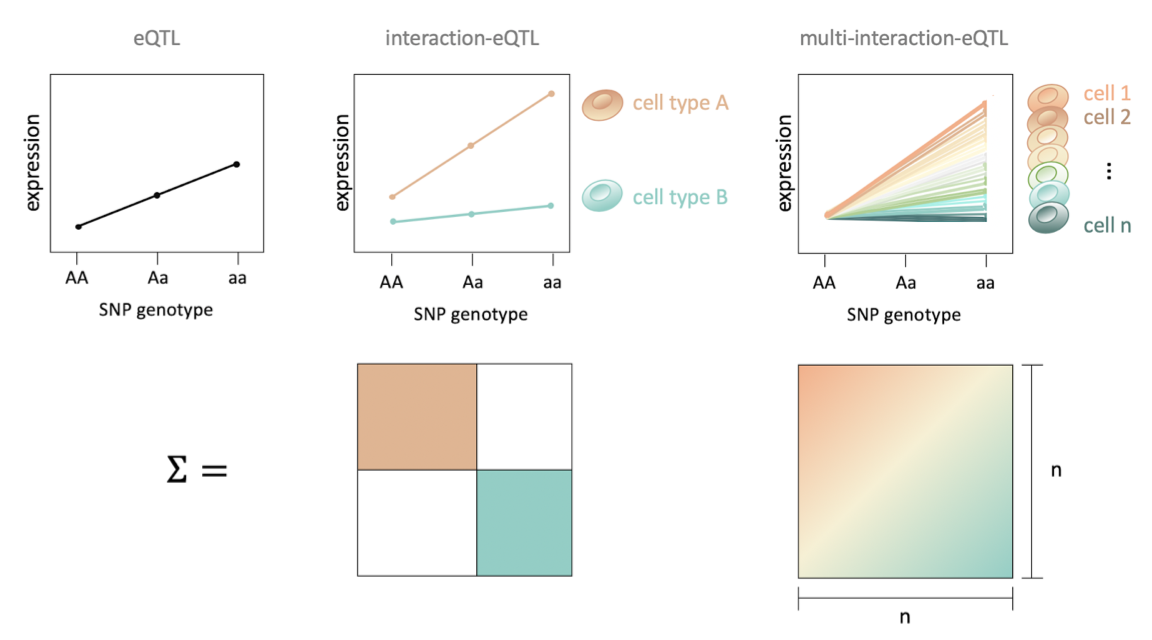
\includegraphics[width=15.5cm]{Chapter6/Fig/sc_structlmm_overview.png}
% \caption[Overview of sc-StructLMM]{\textbf{Overview of sc-StructLMM}.\\
% Think about how to make this figure.}
% \label{fig:sc_structlmm_overview}
% \end{figure}

% \clearpage

\begin{figure}[htbp]
\centering
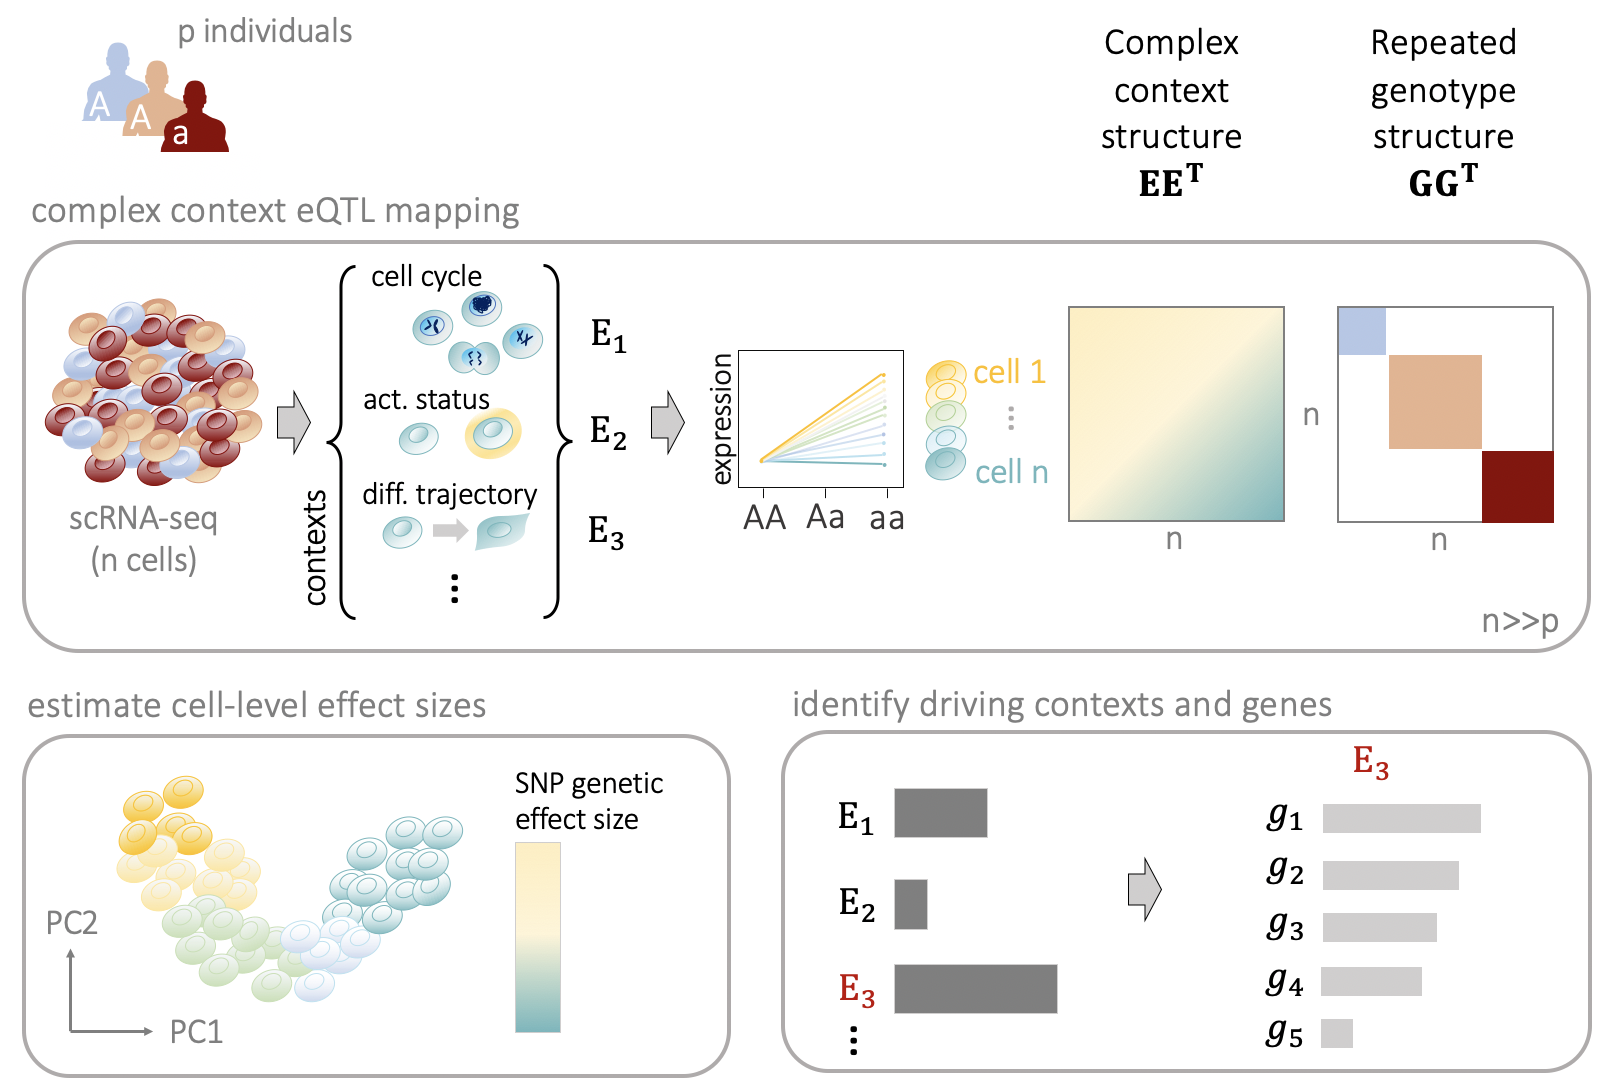
\includegraphics[width=15.5cm]{Chapter6/Fig/sc_structlmm_overview2.png}
\caption[Overview of sc-StructLMM]{\textbf{Overview of sc-StructLMM}.\\
Population-scale scRNA-seq data allows to estimate a number of cellular states and types and then map eQTL across the contexts.
We use a linear mixed model framework which simultaneously takes care of the complex context-structure and the repeatedness (cells per donor) as well as population structure.
Downstream analysis includes the estimation of cell-specific effect sizes driven by GxE, and identification of driving contexts and genes.}
\label{fig:sc_structlmm_overview}
\end{figure}



\clearpage

\section{The sc-StructLMM model} 

As we have seen (\textbf{Chapters 
% \ref{chapter2}-\ref{chapter5}
2-5}), commonly used methods for eQTL mapping fit linear or linear mixed models (LMMs),  whereby a given variant is tested for association with expression changes of a target gene \cite{kilpinen2017common}. 
The effect size is assumed to be shared (persistent) across individuals, or alternatively a discrete group structure (e.g. tissues) can be accounted for \cite{fusi2012joint}. 
In contrast, scStructLMM borrows concepts from the previously described StructLMM model designed for global phenotypes \cite{moore2019linear}, whereby heterogeneity in effect sizes is defined by an environmental (context) covariance matrix, which can capture arbitrary sub-structure in cellular states. 
Specifically, scStructLMM generalises the previous approach by including one additional random effect, which enables to  account for two distinct sets of additive random effect components: population structure as well as cellular context structure.
In particular, accounting for the samples' population structure is critical, as it allows to model not only relatedness and population stratification (\textbf{section 
% \ref{sec:linear_mixed_models}
2.3}), but also replicated measurements for the same donor, in particular the intrinsic repeat structure of single-cell eQTL studies where multiple cells are sampled form the same individual. 
The model can be cast as:

\begin{equation}\label{eq:scStructLMM}
 \mathbf{y} =  \mathbf{W}\boldsymbol{\alpha} + \mathbf{g}\beta_G + \mathbf{g} \odot \boldsymbol{\beta_{GxE}} + \mathbf{e} + \mathbf{u} + \boldsymbol{\psi}, 
\end{equation}

% where $\mathbf{e} \sim \mathcal{N}\mathbf{0},\sigma_e^2 \mathbf{E}\mathbf{E}^T)$, $\mathbf{u} \sim \mathcal{N}\mathbf{0},\sigma_g^2 \mathbf{G}\mathbf{G}^T)$ and $\boldsymbol{\psi} \sim \mathcal{N}\mathbf{0},\sigma_n^2 \mathbf{I_N})$.\\

where $\beta_G$ denotes the effect size of a conventional persistent genetic effect component, and $\boldsymbol{\beta_{GxE}}=[\beta_{GxE_1}, .. ,\beta_{GxE_N}]^T$ is a vector of per-cell effect sizes to account for heterogeneous genetic effects, which follows a multivariate normal distribution, 
% $\boldsymbol{\beta_{GxE}} \sim \mathcal{N}(\mathbf{0},\sigma_{GxE}^2 \mathbf{E}\mathbf{E}^T)$. 
$\boldsymbol{\beta_{GxE}} \sim \mathcal{N}(\mathbf{0},\sigma_{GxE}^2 \boldsymbol{\Sigma})$. 
Depending on the functional form of the environmental covariance, this model can account for different types of G$\times$E, for example, both discrete and continuous cell states and types or donor-level environmental covariates. 
The same environmental covariance is also used to account for additive environmental effects, 
% $\mathbf{e} \sim \mathcal{N}(\mathbf{0},\sigma_e^2 \mathbf{E}\mathbf{E}^T)$ 
$\mathbf{e} \sim \mathcal{N}(\mathbf{0},\sigma_e^2 \boldsymbol{\Sigma})$ 
\cite{moore2019linear}. 
Finally, additive global genetic effects are accounted for using a relatedness matrix ($\mathbf{R}$) (calculated using PLINK \cite{purcell2007plink}, see \textbf{section 
% \ref{sec:linear_mixed_models}
2.3.2}), such that
$\mathbf{u} \sim \mathcal{N}(\mathbf{0},\sigma_g^2 \mathbf{R})$,
% $\mathbf{u} \sim \mathcal{N}(\mathbf{0},\sigma_g^2 \mathbf{G}\mathbf{G}^T)$,
appropriately expanded to reflect the repeated structure of multiple cells derived from the same donors (\textbf{Fig. \ref{fig:sc_structlmm_expanded}}). \\

Similar to models described before, $\mathbf{y}$ represent the $N \times 1$ expression phenotype vector (noting that $N$ is the number of cells, not donors); $\mathbf{W}$ are known covariates, and $\boldsymbol{\alpha}$ the corresponding weights.
In particular, cellular covariates (i.e. observations made at cell level), can be included as columns of $\mathbf{W}$ as they are, whereas donor-level covariates (e.g. sex, age) will need to be expanded first.
Similarly, the genotype vector $\mathbf{g}$ is expanded to fit the model (\textbf{Fig. \ref{fig:sc_structlmm_expanded}}).
Finally, the noise term is gaussian and i.i.d. $\boldsymbol{\psi} \sim \mathcal{N}(\mathbf{0},\sigma_n^2 \mathbf{I_N})$.\\

\begin{figure}[h]
\centering
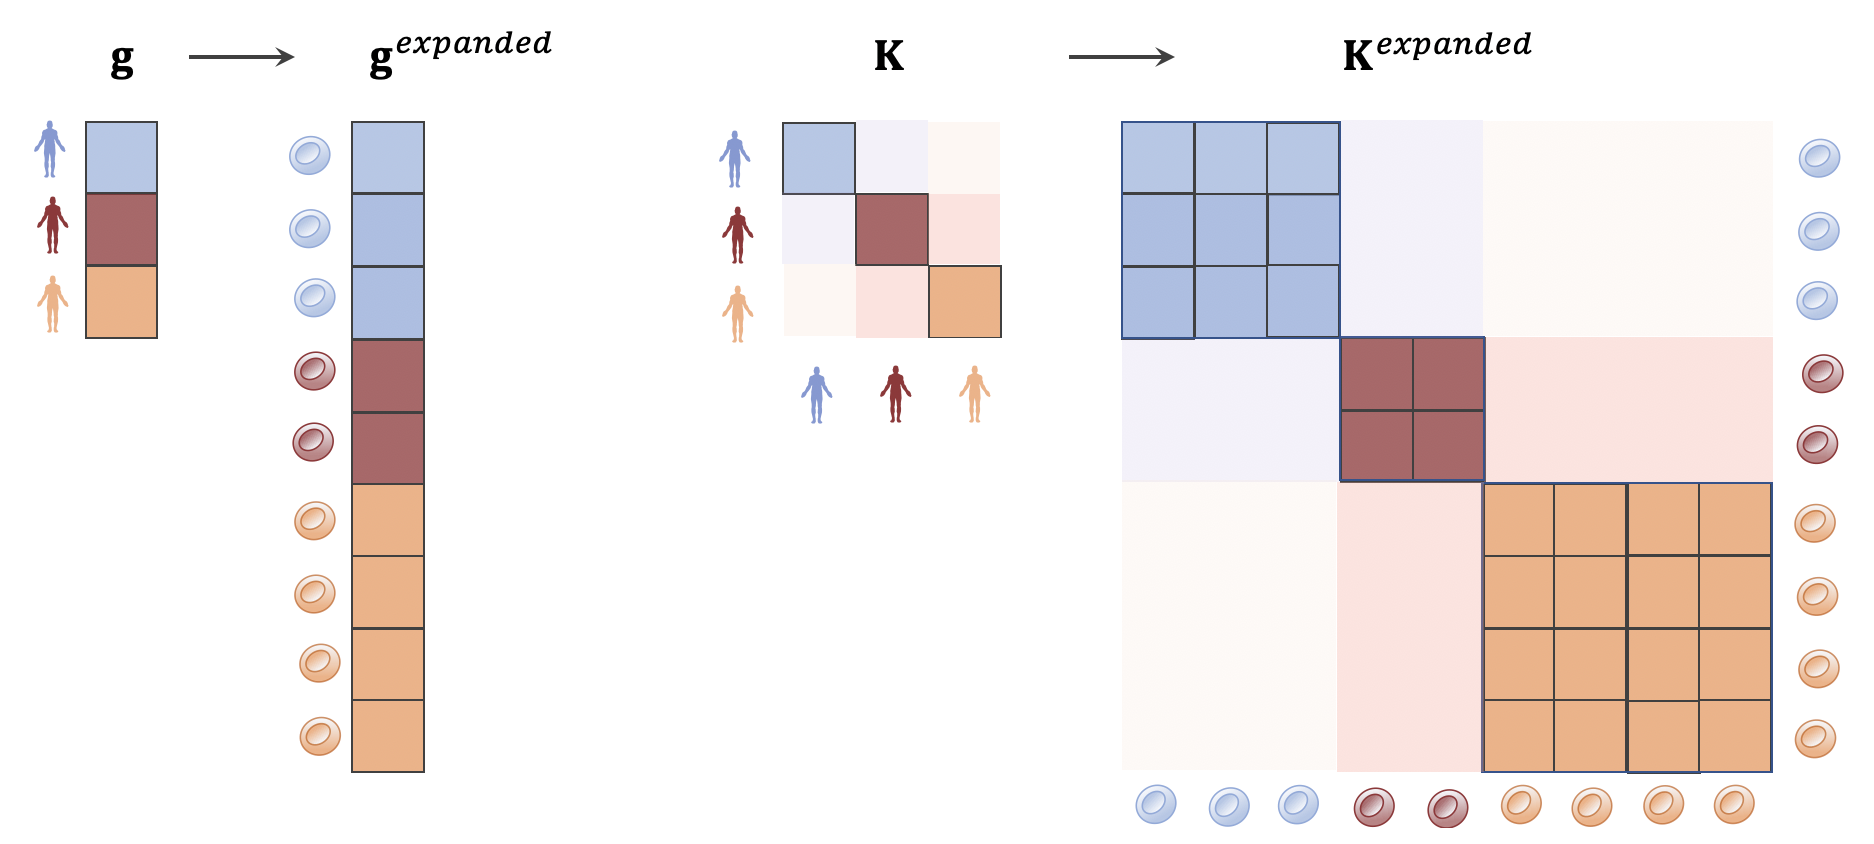
\includegraphics[width=15.5cm]{Chapter6/Fig/sc_structlmm_expanded.png}
\caption[Schematic of expanded genotype vector and kinship matrix]{\textbf{Schematic of expanded genotype vector and kinship matrix}.\\
Schematic of `expansion' from donor-level to cell-level.
Similar as to what is illustrated in \textbf{Fig. \ref{fig:kinship_repeats}}, except we have to deal now with hundreds of cells per donor, rather than 2 or 3 experimental replicates.}
\label{fig:sc_structlmm_expanded}
\end{figure}

% \newpage

The statistical test to be performed evaluates the significant contribution of the GxE component (i.e. $\sigma_{GxE}^2 > 0$)\footnote{This test is equivalent to the StructLMM-int test presented in eq. \eqref{eq:StructLMM-int}.}.
We 
% Because we 
use Rao's Score test (see \textbf{section 
% \ref{sec:hypothesis_testing}
2.2.1}), thus we only need to evaluate the MLE of the parameters 
% likelihood
under $H_0$:

\begin{equation}\label{eq:scStructLMM_H0}
 \mathbf{y}|H_0 =  \mathbf{W}\boldsymbol{\alpha} + \mathbf{g}\beta_G + \mathbf{e} + \mathbf{u} + \boldsymbol{\psi} 
\end{equation}

\begin{equation}\label{eq:scStructLMM_H0_MVN}
 \mathbf{y}|H_0 \sim \mathcal{N}( \mathbf{W}\boldsymbol{\alpha} + \mathbf{g}\beta_G, \sigma_e^2 \mathbf{E}\mathbf{E}^T + \sigma_g^2 \mathbf{G}\mathbf{G}^T+ \sigma_n^2 \mathbf{I} )
\end{equation}

Now, to be able to use the trick described in \textbf{section 
% \ref{sec:fast_lmm},
2.3.3}, 
we need to write the covariance matrix in the form $\sigma^2(\mathbf{M}+\delta\mathbf{I})$ as in eq.
\eqref{eq:fast_lmm_full_covariance}.
% 2.39.
To do so, we introduce a weight parameter $\rho_1$ such that the covariance matrix of $\mathbf{y}$ under the null hypothesis, $\mathbf{K}_0 = \mathrm{Var}(\mathbf{y} | H_0)$ can be re-written as:

\begin{equation}
\begin{split}
    \mathbf{K}_0 = \sigma_e^2 \mathbf{E}\mathbf{E}^T + \sigma_g^2 \mathbf{G}\mathbf{G}^T+ \sigma_n^2 \mathbf{I} =\\
    \sigma_k^2[\rho_1\mathbf{E}\mathbf{E}^T + (1-\rho_1) \mathbf{G}\mathbf{G}^T] + \sigma_n^2 \mathbf{I} =\\ \sigma_k^2\{\boldsymbol{\Sigma}(\rho_1) + \delta_1 \mathbf{I}\},
\end{split}
\end{equation}

where $\sigma_k^2\rho_1 = \sigma_e^2$,
$\sigma_k^2(1-\rho_1) = \sigma_g^2$,
$\delta_1 = \sigma_n^2/\sigma_k^2$, and $\boldsymbol{\Sigma}(\rho_1) = \rho_1\mathbf{E}\mathbf{E}^T + (1-\rho_1) \mathbf{G}\mathbf{G}^T$.\\

I note that $\boldsymbol{\Sigma}$ only depends on $\rho_1$. 
To efficiently implement this, we perform a grid search over $\rho_1$ with as little as 10 possible values (from 0 to 1), thus only slowing down the original method by a factor of 10.

\section{Statistical testing}

To test for GxE interactions we apply the same strategy that is used in the StructLMM method, which in turn adopts the strategy described in Lippert et al \cite{lippert2011fast}.
% Rao et al \cite{rao1948large}.
I use this section to describe the key steps involved.
First, we define the score-based test statistic $\mathrm{Q}$ as:

\begin{equation}\label{eq:Q}
    \mathrm{Q} = \frac{1}{2}\mathbf{y}^T\mathbf{P}_0 \frac{\partial \mathbf{K}}{\partial \theta}\mathbf{P}_0 \mathbf{y}, 
\end{equation}

where $\mathbf{K}$ is the full covariance matrix (from eq. \eqref{eq:scStructLMM}):

% \begin{equation}\label{eq:full_K_scStructLMM}
%     \mathbf{K} = \sigma_{GxE}^2\mathrm{diag}(\mathbf{g})\mathbf{E}\mathbf{E}^T\mathrm{diag}(\mathbf{g}) +  \sigma_e^2 \mathbf{E}\mathbf{E}^T + \sigma_g^2 \mathbf{G}\mathbf{G}^T+ \sigma_n^2 \mathbf{I}
% \end{equation}

\begin{equation}\label{eq:full_K_scStructLMM}
    \mathbf{K} = \sigma_{GxE}^2\mathrm{diag}(\mathbf{g})\boldsymbol{\Sigma} \ \mathrm{diag}(\mathbf{g}) +  \sigma_e^2 \boldsymbol{\Sigma} + \sigma_g^2 \mathbf{G}\mathbf{G}^T+ \sigma_n^2 \mathbf{I}
\end{equation}

and 

\begin{equation}
    \mathbf{P}_0 = \mathbf{K}_0^{-1}-\mathbf{K}_0^{-1}\mathbf{X}(\mathbf{X}^T\mathbf{K}_0^{-1}\mathbf{X})^{-1}\mathbf{X}^T\mathbf{K}_0^{-1}
\end{equation}

is a matrix that projects out the fixed effects \cite{lippert2011fast, lippert2014greater}.
In our case (eq. \eqref{eq:scStructLMM}), the fixed effects include covariates and the persistent effect of the variant tested: $\mathbf{X} = [\mathbf{W}, \mathbf{g}]$\\

Using eq. \eqref{eq:full_K_scStructLMM} and considering the parameter $\theta = \sigma_{GxE}^2$, we can derive:

% \begin{equation}
%     \frac{\partial \mathbf{K}}{\partial \sigma_{GxE}^2} = \mathrm{diag}(\mathbf{g})\mathbf{E}\mathbf{E}^T\mathrm{diag}(\mathbf{g}).
% \end{equation}

% Next, let us define $\mathbf{K}_1 = \mathrm{diag}(\mathbf{g})\mathbf{E}\mathbf{E}^T\mathrm{diag}(\mathbf{g})$and substituting in eq. \eqref{eq:Q}, we can write:

\begin{equation}
    \frac{\partial \mathbf{K}}{\partial \sigma_{GxE}^2} = \mathrm{diag}(\mathbf{g})\boldsymbol{\Sigma} \ \mathrm{diag}(\mathbf{g}).
\end{equation}

Next, let us define $\mathbf{K}_1 = \mathrm{diag}(\mathbf{g})\boldsymbol{\Sigma} \ \mathrm{diag}(\mathbf{g})$and substituting in eq. \eqref{eq:Q}, we can write:

\begin{equation}
    \mathrm{Q} = \frac{1}{2}\mathbf{y}^T\mathbf{P}_0 \mathbf{K}_1\mathbf{P}_0 \mathbf{y} 
\end{equation}

As in eq. \eqref{eq:StructLMM-int_H1}, $H_1: \sigma_{GxE}^2>0$, noting that as a variance parameter, $\sigma_{GxE}^2$ can only take positive values.
As a result, the score test statistic $\mathrm{Q}$ does not follow the usual $\chi^2_i$ distribution (see eq. \eqref{eq:lagrange_multiplier_univariate}), but instead a mixture of  $\chi^2$ distributions.
I refer the reader specifically at the supplementary methods from \cite{lippert2014greater} for a proof.

\begin{equation}
    \mathrm{Q} \sim \sum_i \lambda_i \chi^2_1 
\end{equation}

Where $\lambda_i$'s are the non-zero eigenvalues of $\frac{1}{2}\mathbf{P}_0^{\frac{T}{2}} \frac{\partial\mathbf{K}}{\partial \theta} \mathbf{P}_0^{\frac{1}{2}}$.\\

It can be shown that for a matrix $\mathbf{A}$ the eigenvalues of $\mathbf{A}\mathbf{A}^T$ are the same as those of $\mathbf{A}^T\mathbf{A}$ , this we can re-arrange and compute $\lambda_i$'s as the eigenvalues of:

\begin{equation}
    \frac{1}{2}\frac{\partial\mathbf{K}}{\partial \theta}^{\frac{T}{2}} \mathbf{P}_0 \frac{\partial\mathbf{K}}{\partial \theta}^{\frac{1}{2}},
\end{equation}

instead.

To evaluate the significance of the score-best test statistic $\mathrm{Q}$ we use the approach described in SKAT \cite{wu2011rare}, thereby using the Davies exact method \cite{davies1980algorithm} to compute the corresponding p values, and switching to the modified moment matching approximation method \cite{liu2009new, lee2012optimal, duchesne2010computing} when this fails to converge.


% Various methods have been proposed to compute the tail probability of the mixture of 1-dof $\chi^2$ distributions. 
% For example, we can use the Davies method \cite{davies1980algorithm}, the moment‐matching‐based noncentral $\chi^2$ approximation method \cite{liu2009new, lee2012optimal}, or the saddlepoint approximation method \cite{kuonen1999miscellanea}. 
% The Davies methos is the most accurate but can be be computationally expensive.
% The moment-matching approximation is anti-conservative and could lead to inflated type I errors especially for small significance levels.
% SKAT: Davies + Liu
% SKATh: Davies + saddle
% \cite{wu2016efficient}

% \section{Definition of covariance matrix}

% E?

% PCs, MOFA, HVGs?
% transformation?
% normalisation/scaling



% \section{Application to simulated data}

% % First, we applied the model on simulated data.

% First, I used simulation experiments to show calibration (see \textbf{section 
% % \ref{sec:confounders}
% 2.2.4}) of scStructLMM is calibrated.
% % , and then to demonstrate the 
% % power 
% % advantages of scStructLMM compared to other methods. 
% % forthe interaction and association test (Section 2.3). 
% I use this section to describe the simulation procedure used to generate these simulated data and the methods used to assess calibration.
% % and statistical power. 
% % I will then show calibration and power results for some general settings, followed by results for simulation experiments that explicitly examine the effect of certain environmental properties.

% \subsection{Simulation strategy}

% \subsubsection{Genotype data}

% Given $S$ number of SNPs, I first generated $S$ random minor allele frequencies (MAFs) between 0.1 and 0.45.
% Given those, and a number of donors $N$, I generated $S$ independent $N \time 1$ $\mathbf{g}$ vectors as random vectors of 0, 1, 2 with probabilities given by the corresponding MAF ($p(2) = MAF^2$, $p(0) = (1-MAF)^2$, and $p(1) = 1 - p(0) - p(2)$).  

% \subsubsection{Kinship matrix}

% Next, I defined the IBD matrix as the $N \times N$ matrix $\mathbf{R} = \mathbf{G}\mathbf{G}^T$, where $\mathbf{G}$ is the $N \times S$ genotype matrix from above.
% $\mathbf{R}$ was then column-normalised.

% \subsubsection{Environments}

% First, I define the context covariance matrix as:
% $\boldsymbol{\Sigma} = \mathbf{E}\mathbf{E}^T$.

% Next, I simulated two different types of context covariance matrix.

% \subsubsection{Phenotype}

% Briefly, from the full model (eq. 6.1) we simulate only an intercept as covariate, such that:  

% \begin{equation}
%  \mathbf{y} = \mathbf{y}_0 + \mathbf{g}\beta_G + \mathbf{g} \odot \boldsymbol{\beta_{GxE}} + \mathbf{e} + \mathbf{u} + \boldsymbol{\psi}, 
% \end{equation}

% where I column-normalise all terms so that the total variance sums to 1.
% Next, I set the variance explained by both genetic terms $var_G+var_{GxE}=\sigma_0^2$, and call the rest $v = 1-\sigma_0^2$.

% Further, I regulate the amount of variance driven by GxE using an additional weighting factor $\rho_0$, such that: $var_G = (1-\rho_0)\sigma_0^2$ and $var_{GxE} = \rho_0\sigma_0^2$
% For simplicity, I set the variances explained by the last three terms to be the same:
% $\sigma_E^2 = \sigma_g^2 = \sigma_n^2 = v/3$. \\

% More specifics on how I simulate the betas, and how i set the variance explained to whatever value.

% \subsection{Calibration analysis}

% Using the data simulated as above, I first checked whether the model was calibrated both in the case of no genetic effects at all (i.e. $\sigma_0^2 = 0$) and in the case of persistent effects only (no GxE, i.e. $\rho_0 = 0$) (\textbf{Fig. \ref{fig:sc_structlmm_calibration}}).
% Specify number of donors, cells, snps used here.

% \begin{figure}[h]
% \centering
% 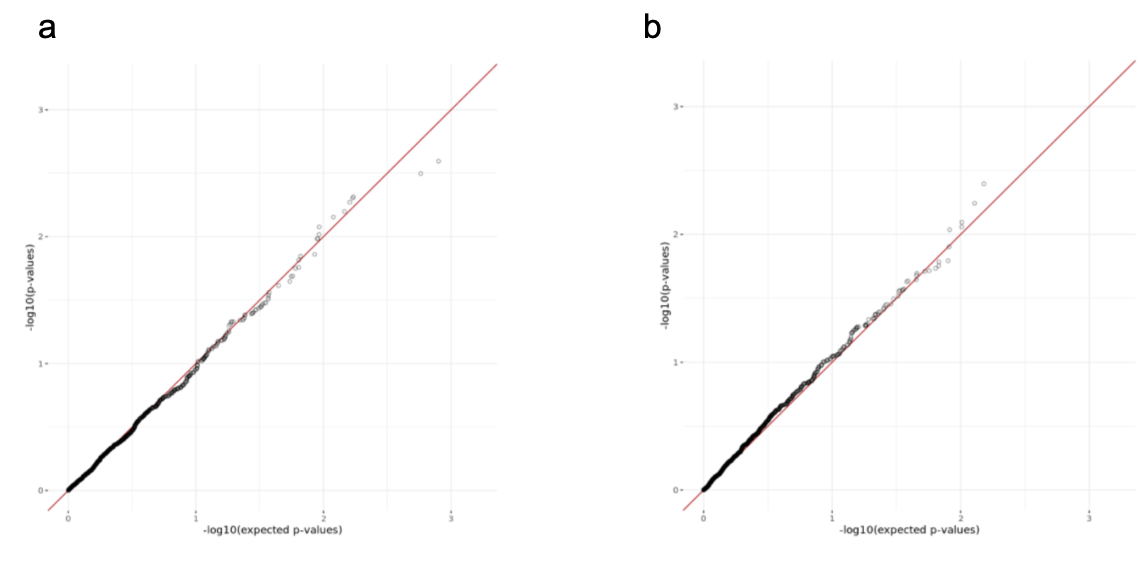
\includegraphics[width=15.5cm]{Chapter6/Fig/sc_structlmm_calibration.png}
% \caption[Calibration QQ-plots]{\textbf{Calibration QQ-plots}.\\
% (a) No genetic effect at all.
% (b) No GxE effect (persistent only).}
% \label{fig:sc_structlmm_calibration}
% \end{figure}

% % \subsection{Comparison with Struct LMM v0}

% % Next, we compared our model to the original StructLMM model.
% % StructLMM is expected to have issues in the presence of extended repeated structure, which it is not equipped to deal with.
% % To address this, we simulated various numbers of repeats per donor - mimicking cells -  ranging from 10 to 500.
% % Indeed, we observe over-inflation of StructLMM in the presence of many repeats making the model not calibrated (Fig. Xa).
% % sc-StructLMM, on the other hand, is nicely calibrated (Fig. Xb).

% % \subsection{Comparison with standard interaction test}

% % We then performed power analysis when comparing our model with one where the environments are modelled as fixed effects (see Section 2.4.2).

% \clearpage

% \section{Real data}
\section{Application to differentiating iPS cells}

% Next, 
I applied sc-StructLMM on the data described in \textbf{Chapter 
% \ref{chapter4}
4} (and published in \cite{cuomo2020single}).
% We applied our model on a recently published dataset.
Briefly, human iPS cells (\textbf{section 
% \ref{sec:ipsc}
1.2}) from 125 donors are differentiated from a pluripotent state, to definitive endoderm. 
% \subsection{Analysis of factors using MOFA}
I use 
% principal components (PCs) 
multi-factor analysis (MOFA \cite{argelaguet2018multi}) to identify factors that
% 10 MOFA factors estimated from the data \cite{argelaguet2018multi}
% 500 independent ($r^2<0.2$) highly variable genes (HVGs)
% to 
capture various aspects of the variation in gene expression in the dataset, which represent cell states and types. 
In particular, the MOFA factor1 aligns with the differentiation axis (similar to PC1, see \textbf{section 
% \ref{sec:endodiff_sources_of_variation}
4.3.1}). 
Factor 3, on the other hand, captures cells in different phases along the cell cycle, as estimated using Seurat \cite{stuart2019comprehensive} (\textbf{Fig. \ref{fig:sc_structlmm_endo_mofa_factors}}). 
\\

\begin{figure}[h]
\centering
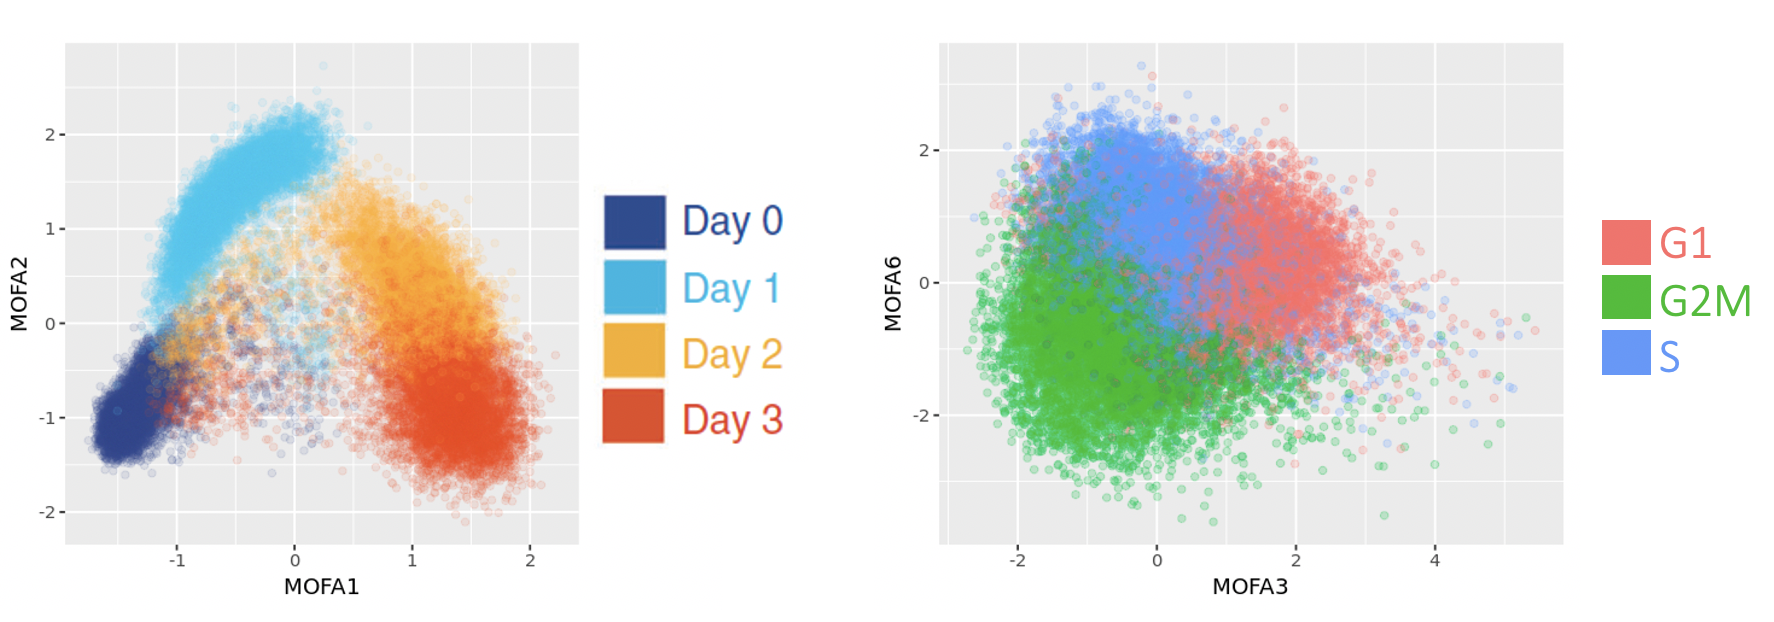
\includegraphics[width=15.5cm]{Chapter6/Fig/MOFA_factors.png}
\caption[MOFA factors used as contexts]{\textbf{MOFA factors used as contexts}.\\
Evaluation of some of the factors identified using multi-omics factor analysis (MOFA \cite{argelaguet2018multi}).
(left) MOFA1 and MOFA2 mostly reflect the developmental stage of our cells, with MOFA1 (x axis) recapitulating a differentiation trajectory from iPSCs (day0) to definitive endoderm (day3).
MOFA3 vs MOFA6: cell cycle.}
\label{fig:sc_structlmm_endo_mofa_factors}
\end{figure}

First, I used the first 10 factors calculated using MOFA as cellular states in the model (i.e. as columns of $\mathbf{E}$ from eq. \eqref{eq:scStructLMM}).
For numerical reasons, the factors were quantile normalised, prior to building the covariance matrix (as $\mathbf{E}\mathbf{E}^T$). 
% \\
Next, I tested the combined set of eQTL identified at any of the developmental stages defined in \textbf{Chapter 
% \ref{chapter4}
4} (iPSC, mesendo, defendo - for a total of 4,470 gene-SNP pairs) for GxE interactions.
Single cell expression of each of the eGenes tesed ($\mathbf{y}$) was also quantile-normalised. \\

To assess the effect of including more cell states in the model, I tested the model using only one factor, the first two factors, the first five, and finally all ten factors (\textbf{Fig. \ref{fig:sc_structlmm_endo_barplots}}).

\newpage

% \subsection{Data prep}

% Both y and E are quantile normalised,..

\subsection{Permutation strategy for multiple testing correction}

To correct for multiple testing correction, I used a permutation approach similar to that described in \cite{ongen2016fast}.
In particular, I ran 100 permutations for each of the eQTL tested, where I permuted the values of the cell states (i.e. the MOFA factors) within each donor, across cells.
Next, for each set of permutations, I select the minimum (permuted) p value, across all eQTL.
I then use these 100 permuted p values to estimate a beta distribution and correct the original real p values.

\subsection{Results}

We observe an increase in our power to identify `interaction eGenes' (i.e. genes with at least one GxE interaction eQTL) as we increase the number of 
factors included as contexts 
% PCs used as environments, with then a plateau at 50 PCs
(\textbf{Fig. \ref{fig:sc_structlmm_endo_barplots}}). \\

\begin{figure}[htbp]
\centering
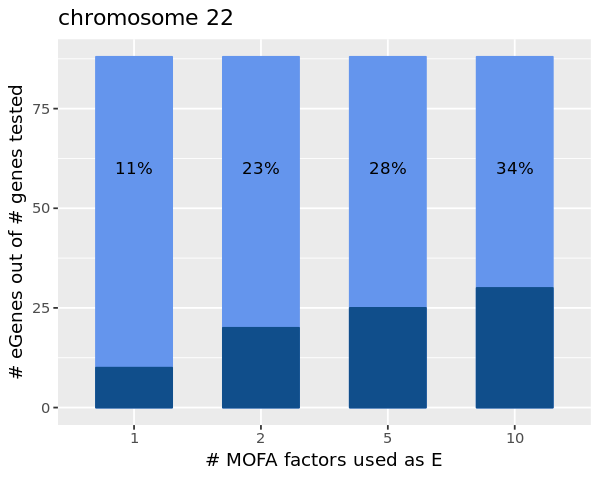
\includegraphics[width=14cm]{Chapter6/Fig/sc_structlmm_endodiff_mofa.png}
\caption[Results on endodiff data]{\textbf{Results on endodiff data}.\\
Barplots showing the number of eGenes compared to the genes tested.
Endodiff significant eGenes only (iPSC+mesendo+defendo, FDR < 10\%).
Chromosome 22 only (88 genes).}
\label{fig:sc_structlmm_endo_barplots}
\end{figure}

% Reassuringly, we could recapitulate most (XX\%) of the dynamic eQTL described in the original study (\textbf{section 
% % \ref{sec:endodiff_dynamic_eqtl}
% 4.5}), which were detected using solely PC1, 
% % and using ASE and a linear model (see eq. \eqref{eq:endodiff_ase_pseudotime}
% % 4.1).
% % and a fixed effect linear mixed model (Methods). 
% However, we show that we have increased power using our model. 
% Furthermore, the overlap with our interaction eQTL and the dynamic eQTL identified in Cuomo \textit{et al}. decreases, the more PCs we include (Fig. XX).\\



% As environments, we used
% the first 10 principal components


% PCs, MOFA, HVGs?
% transformation?
% normalisation/scaling




% \section{Upstream analysis}

% One of the key steps in running this method is choosing the environmental factors.
% We expect most applications to be for scRNA-seq datasets only (and genotypes).
% This means that the environments need to be estimated from the transcriptomic data, which is also used as phenotype, causing concerns of circularity.


% A user might have 
% PCA
% MOFA (single omic)

% \section{Downstream analysis} 
\newpage
% \subsection{Estimate cell-specific genetic effects}
\section{Predicting cell-specific effect sizes driven by GxE}

Using our model it is also possible to estimate a cell-specific genetic effect size due to GxE (thus estimating $\boldsymbol{\beta_{GxE}}$ from eq. \eqref{eq:scStructLMM}) for each gene-SNP pair tested.
Because this is not optimised, we only perform this as downstream analysis, on gene-SNP pairs that pass a significance threshold.\\

Briefly, we note that given a generic gaussian process ($\mathrm{GP}$) of the form:
 
\begin{equation}
    \mathbf{f}(\mathbf{X}) \sim \mathrm{GP}(\mathbf{m}(\mathbf{x}), k(\mathbf{x},\mathbf{x}^T)),
\end{equation}

the best estimator of the out-of-sample prediction for $\mathbf{f}_*$  is its best linear unbiased predictor (BLUP), defined as its expected value condition on $\mathbf{f}$ and $\mathbf{X},\mathbf{X}_*$:

\begin{equation}
    E[\mathbf{f}_*|\mathbf{f}] = \mathbf{m}_* +k(\mathbf{X}_*,\mathbf{X})k(\mathbf{X},\mathbf{X})^{-1}(\mathbf{f}-\mathbf{m}).
\end{equation}

In our case,

\begin{equation}
    \mathbf{f}(\mathbf{X}) = \mathbf{y} = \mathbf{W}\boldsymbol{\alpha}+\mathbf{g}\beta_G+\mathbf{g}\boldsymbol{\beta}_{GxE}+\mathbf{e} + \mathbf{u} + \boldsymbol{\psi},
\end{equation}

with ($\mathbf{X} = {\mathbf{W},\mathbf{g},\mathbf{E},\mathbf{K}}$) such that:

\begin{equation}
    \mathbf{m}(\mathbf{X}) = \mathbf{W}_*\boldsymbol{\alpha}_{*}+\mathbf{g}_*\beta_G
\end{equation}

\begin{equation}
    k(\mathbf{X},\mathbf{X}) = \sigma_{GxE}^2(\mathbf{g}\odot\mathbf{E})(\mathbf{g}\odot\mathbf{E})^T
\end{equation}

and 

\begin{equation}
\mathbf{y}_{*}^{BLUP} = E[\mathbf{y}_*|\mathbf{y}] = \mathbf{W}_*\boldsymbol{\alpha}_{*}+\mathbf{g}_*\beta_G+\mathbf{E}_*\gamma + k(\mathbf{X}_*\mathbf{X})K^{-1}(\mathbf{y}-\mathbf{W}\boldsymbol{\alpha}-\mathbf{g}\beta_G-\mathbf{E}\gamma).
\end{equation}

and how do you go from here to beta gxe?

\newpage
% \clearpage



We perform this analysis only for the subset of XXX eQTL that exhibit some GxE effects (FDR < 10\%).
Reassuringly, we see that Oct4, .. (\textbf{Fig. \ref{fig:sc_structlmm_pcas}}).\\

\begin{figure}[htbp]
\centering
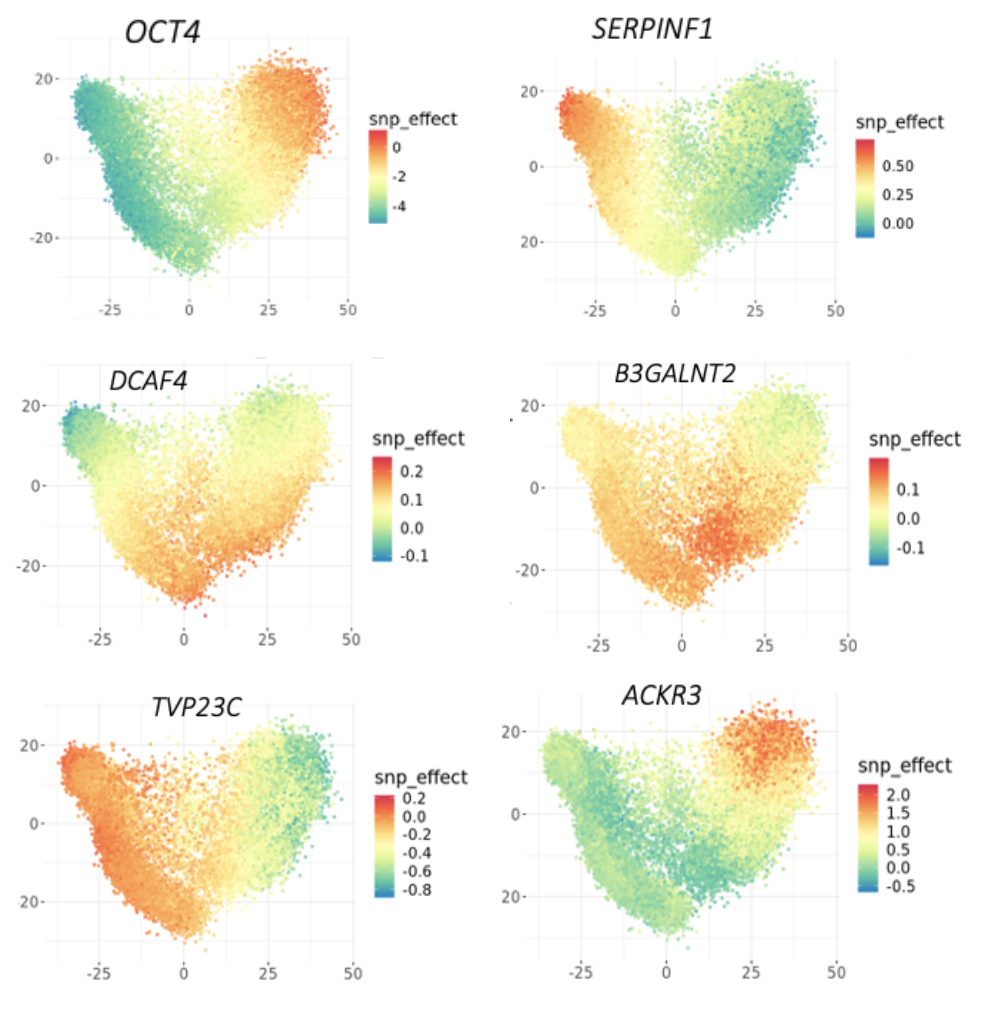
\includegraphics[width=15.5cm]{Chapter6/Fig/sc_structlmm_pcas.png}
\caption[Cell-specific effect sizes]{\textbf{Cell-specific effect sizes}.\\
PCA plots representing exemplar eQTL affected by GxE.
Cells are coloured by estimated effect sizes.}
\label{fig:sc_structlmm_pcas}
\end{figure}

\clearpage

One important axis of variation is time, thus we cluster using Palantir \cite{setty2019characterization}
(\textbf{Fig. \ref{fig:sc_structlmm_clusters}}).

\begin{figure}[h]
\centering
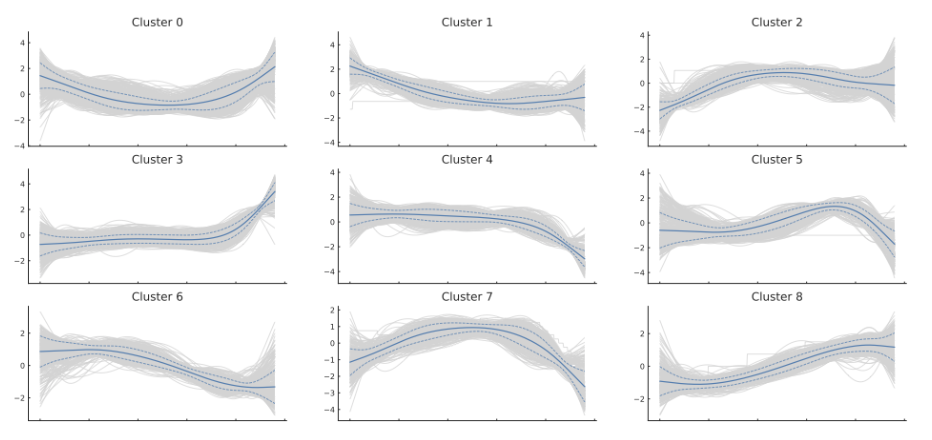
\includegraphics[width=15.5cm]{Chapter6/Fig/sc_structlmm_clusters.png}
\caption[Clusters of dynamic eQTL]{\textbf{Clusters of dynamic eQTL}.\\
Clusters using Palantir.}
\label{fig:sc_structlmm_clusters}
\end{figure}

\clearpage

\section{Discussion}

Here, I have presented a method that allows for the joint testing of multivariate context-specific eQTL mapping across cellular states and types, as estimated from single cell RNA-seq expression profiles.\\

In particular, the method is able to .. (\textbf{Fig. \ref{fig:sc_structlmm_overview}})

Next..

I have shown preliminary results on simulated data, showing calibration and..\\

This work is still in early stages, with significant work still to do to validate the results...
Address things still to do 
run on 10x data
validate results
explore more \\

One of the key steps in running this method is choosing the environmental factors, prior to testing the method.
We expect most applications to be for scRNA-seq datasets only (and genotypes).
This means that the environments need to be estimated from the transcriptomic data, which is also used as phenotype, causing concerns of circularity.\\

On the other hand, downstream analysis steps may include methods to determine which of the included environments are responsible..\\

A limitation of the model is that it models the phenotype vector (single cell expression profile of a genes) as following a normal distribution.
We quantile-normalise y, which makes a difference, but future work should include extension to non-Gaussian likelihoods (e.g. Poisson, Negative Binomial).
However, GLMMs are slow..\\

Finally, while the main application of the method is single cell context-specific eQTL mapping across several states, this model is in principle flexible to any application with repeat measurements for the same individual (e.g. longitudinal data)
% \begin{itemize}
%     \item GLMM (Poisson, NB)
%     \item additional covariances?
%     \item other applications (longitudinal data)
% \end{itemize}
